% Generative adversarial network (GAN) architecture.
% Adapted from https://github.com/PetarV-/TikZ/tree/master/Generative%20adversarial%20network.
% A GAN has two parts. The discriminator $D$ acts as a classifier that learns to distinguish fake data produced by the generator $G$ from real data. $G$ incurs a penalty when $D$ detects implausible results. This signal is backpropagated through the generator weights such that $G$ learns to produce more realistic samples over time, eventually fooling the discriminator if training succeeds.

\documentclass[tikz]{standalone}

\usepackage{mathtools}

\usetikzlibrary{calc,positioning}

\begin{document}
	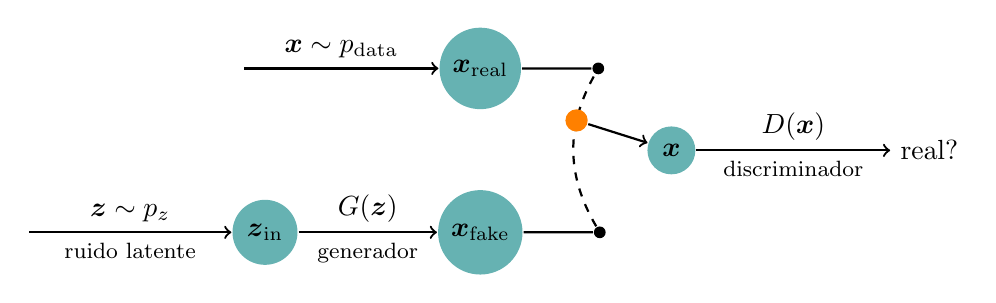
\begin{tikzpicture}[
		->, thick,
		node/.style={circle, fill=teal!60},
		label/.style={below, font=\footnotesize},
		]
		
		\node[node] (zin) {$\boldsymbol{z}_\text{in}$};
		\node[node, right=5em of zin] (fake) {$\boldsymbol{x}_\text{fake}$};
		\draw (zin) -- node[above] {$G(\boldsymbol{z})$} node[label] {generador} (fake);
		
		\draw[<-] (zin) -- node[above] {$\boldsymbol{z} \sim p_z$} node[label] {ruido latente} ++(-3,0);
		\node[node, above=of fake] (real) {$\boldsymbol{x}_\text{real}$};
		\draw[<-] (real) -- node[above] {$\boldsymbol{x} \sim p_\text{data}$} ++(-3,0);
		\node[node, right=6em of fake] (D) at ($(fake)!0.5!(real)$) {$\boldsymbol{x}$};
		\node[right=7em of D] (out) {real?};
		\draw (D) -- node[above] {$D(\boldsymbol{x})$} node[label] {discriminador} (out);
		
		\coordinate[right=2.5em of fake, circle, fill, inner sep=0.15em] (pt1);
		\coordinate[right=2.5em of real, circle, fill, inner sep=0.15em] (pt2);
		
		\draw[-, dashed] (pt1) edge[bend left] coordinate[circle, fill=orange, inner sep=1mm, pos=0.7] (pt3) (pt2);
		\draw (fake) -- (pt1) (real) -- (pt2) (pt3) -- (D);
		
	\end{tikzpicture}
\end{document}